%%%%%%%%%%%%%%%%%%%%%%%%%%%%%PREÁMBULO DEL DOCUMENTO%%%%%%%%%%%%%%%%%%%%%%%%%%%
% En esta sección se configura el document, pero no se incluye contenido
% Esto es la clase del documento, que defines las instrucciones principales
% que condicionarán el documento generado. Generalmente cambiarla después de 
% añadir contenido produce numerosos errores.
\documentclass{article}

%%%%%%%%%%%%%%%%%%%SECCIÓN INCLUSIÓN DE PAQUETES %%%%%%%%%%%%%%%%%%%%%%%%%%%%%%
% Carga el paquete babel, las opciones son:
    % spanish: indica que usaremos configuración para escribir en español
    % es-tabla: traduce la palabra table como tabla, no como cuadro
    % es-lcroman: permite la numeración romanda en minúscula.
\usepackage[spanish, es-tabla, es-lcroman]{babel}
% Paquete que permite escribir el símbolo del euro, se usa de dos maneras.
    % En el documento, la orden \euro escribirá el símbolo
    % Si se escribe \EUR{<cifra>} el paquete formará un bloque con el
        % número y el símbolo.
\usepackage{eurosym} 
% Paquete para que las imágenes tengas un tamaño relativo al del párrafo
\usepackage{graphicx}
% nos permite insertar las figuras con el especificador H, que hace que se
    % inserte en el lugar del document donde se ha escrito su código.
\usepackage{float} 
% Paquete que habilita las referencias cruzadas.
\usepackage{hyperref}
% Permite poner pies y encabezados de página personalizados
\usepackage{fancyhdr}
 %permite referenciar la última página (para incluir páginas totales)
\usepackage{lastpage}
%%%%%%%%%%%%%%%%%%%% FIN SECCIÓN %%%%%%%%%%%%%%%%%%%%%%%%%%%%%%%%%%%%%%%%%%%%%%


% Esta línea nos permite indicar un directorio donde estamos guardando
% nuestras imágenes. Más información más adelante.
\graphicspath{{./img/}}


% Esto hace que los enlaces a webs (\href{url}{texto} salgan en azul.
    % También impide que salga un repugnante rojo alrededor de cada
    % referencia cruzada que incluyas en el documento.
\hypersetup{
    colorlinks=true,
    linkcolor=black,
    filecolor=magenta,      
    urlcolor=blue,
}
% Permite que en las ecuaciones escribas un punto y salga un punto (no lo
% interprete como un decimal en español, es decir, una coma)
\decimalpoint

%%%%%%%%%%%%%%%%%SECCIÓN VARIABLES %%%%%%%%%%%%%%%%%%%%%%%%%%%%%%%%%%%%%%%%%%%%
% Podemos definir variables para usar a lo largo del texto
% Así podemos cambiarlas aquí sin tener que repetir texto.
\def \autor{Autor Autórez Ejémplez}
\def \titulo{Ejemplo de documento en \LaTeX}
\def \organizacion{Universidad de Ejemplo}
%%%%%%%%%FIN SECCIÓN%%%%%%%%%%%%%%%%%%%%%%%%%%%%%%%%%%%%%%%%%%%%%%%%%%%%%%%%%%%

% Esta orden especifica que cuando se cree la portada se use este título.
% Además, con Huge utilizamos la macro de tipo de letra más grande que hay 
% disponible.
\title{\textbf{\Huge{\titulo}}}
% Aquí lo mismo, pero con el autor
% Algunos especificadores de tamaño son: tiny, small, large, Large, LARGE, huge
    % y Huge
\author{\LARGE{\autor}\\ \\ \Large{\organizacion}}
%%%%%%%%%%%%%%%%%%%%%%%%%%%%FIN DEL PREÁMBULO%%%%%%%%%%%%%%%%%%%%%%%%%%%%%%%%%%


%%%%%%%%%%%%%%%%%%%%%%%%%%%%%%INICIO DEL DOCUMENTO%%%%%%%%%%%%%%%%%%%%%%%%%%%%%
% La totalidad del texto que se renderizará en PDF en tu documento debe estar
% entre begin document y end document.
\begin{document}
% Elimina la numeración de página hasta que se diga lo contrario.
\pagenumbering{gobble}
% Pone el título, el autor y la fecha. (la fecha se detecta automáticamente)
\maketitle

% Aquí creamos una figura para poner el logo de algo (Ahora hay un placeholder) 
% más en cuanto a figuras más adelante.
\begin{figure}[H]
% Lo centramos
\center

\includegraphics[width=.5\linewidth]{escudo}
\end{figure}
\newpage
% En esta página puedes poner agradecimientos o prefacios que no tendrán pie ni
% encabezado de página y que no afectarán a la numeración, si no quieres poner
% nada, elimina esta línea y uno de los newpages
\textbf{[Esta página ha sido dejada en blanco a propósito por el editor]}
\newpage
%Vamos a poner agradecimientos
\begin{flushright}
\textit{Esto es un placeholder, muchas gracias, placeholder.}
\end{flushright}
\newpage % salto de página

%%%%%%%%%%%%%%%%% CABECERA Y PIE DE PÁGINA SECCIÓN ÍNDICE%%%%%%%%%%%%%%%%%%%%%
\pagestyle{fancy}
% Incluye una línea horizontal en el encabezado de página.
\fancyhf{}
% Texto de la parte derecha del encabezado, nótese que usamos la variable
    % que hemos definido anteriormente.
\rhead{\autor}
% Texto de la parte izquierda
\lhead{\titulo}
% Incluye el texto "pág. X de Y" en el pie de pág. a la derecha.
    % estoy referenciando una etiqueta que añadí, se verá luego.
\rfoot{pág. \thepage{} de \pageref{startSectionContent}} 
% Incluye una línea en el pie de página.
\renewcommand{\footrulewidth}{0.5pt}
%decimos que se numeren las páginas en romano hasta nueva orden
    % Esto nos permite numerar las páginas de índices en números romanos
\pagenumbering{roman} 
%%%%%%%%%%%%%%%%%FIN
\tableofcontents %crea el índice el índice empieza siempre en página nueva

% se pueden añadir saltos de página extra con \newpage
\newpage

% cambia el nombre del índice de ilustraciones
\renewcommand{\listfigurename}{Índice de ilustraciones}
%inserta el índice de ilustraciones
\listoffigures 
\newpage

%tambia el nombre del índice de tablas
\renewcommand{\listtablename}{Índice de tablas}

%inserta el índice de tablas
\listoftables

% Esta orden (label) inserta etiquetas invisibles en el texto, al ponerla justo
    % antes del salto de página del último índice de la sección, me permite
    % referenciar este punto, así es como consigo que salga "Pág. i de iiii".
\label{startSectionContent}

\newpage

%%%%%%%%%%%%%%%%% CABECERA Y PIE DE PÁGINA SECCIÓN CUERPO%%%%%%%%%%%%%%%%%%%%%%
\pagestyle{fancy}
\fancyhf{}
\rhead{\autor}
\lhead{\titulo}
% El único cambio es que aquí referencio la última página de verdad.
\rfoot{pág. \thepage{} de \pageref{LastPage}}
\renewcommand{\footrulewidth}{0.5pt}
%%%%%%%%%%%%%%%%%%%%%%%%%%%%%%%%%FIN SECCIÓN%%%%%%%%%%%%%%%%%%%%%%%%%%%%%%%%%%%
% La sección es el primer nivel de título que se permite en esta clase de 
    % documento. Introduce un título de primer nivel
\section{Presentación}
Este documento pretende ser un ejemplo de varias tareas que se suelen realizar
en LaTeX. Se recomienda compilar el código y ver el pdf y el mismo código a la
vez para ver los resultados. En los comentarios del código explico lo que se va
haciendo y qué órdenes son necesarias para crear lo que se ve en el PDF.
Además, incluyo un \textit{script} de compilación mínimo que debería compilar
sin problemas. Los prerrequisitos son:
\begin{itemize}
    \item Sistema operativo GNU/Linux
    \item Herramienta make
    \item Tener \LaTeX{} instalado en el sistema, se puede instalar con la orden
    \begin{verbatim}
$ sudo apt-get install texlive-base texlive-latex-recommended \\
  texlive-latex-extra texlive-full 
    \end{verbatim} En sistemas derivados de Debian. En otras distribuciones, 
por favor, consulte la documentación específica de cómo instalar paquetes de
\textit{software}.
\end{itemize}
\section{Contenido}
% A partir de aquí numeración normal
\pagenumbering{arabic}

% párrafo con texto en distintos formatos, textit es itálita, textbf es 
% negrita, se pueden combinar. texttt es monoespaciada, la uso luego
% Como puedes ver, aunque hay saltos de línea, no son párrafos distintos.
% Para que sean párrafos distintos tiene que haber una línea en blanco
% entre ellos.
Este es el primer párrafo de esta sección, en cualquier texto
podemos incluir texto en
\textbf{negrita} o en \textit{cursiva}, incluso, podríamos incluir texto en 
\textbf{\textit{negrita y cursiva}}. Además de texto, es natural que en un 
documento tengamos que poner lista, ya sean éstas numeradas o sin numerar.
A continuación vemos cómo se hace.

%%% Ejemplo de lista
% Este tipo de listas no son numeradas. Son listas de puntos (bullets)
\begin{itemize}
    % Un item es una fila de la lista, un punto, en este caso.
    \item Sector primario
    % si quieres subniveles, creas una lista dentro de esta.
    % Ojo, cuidado, tiene que haver un item antes, como aquí que está
    % el item sector primario.
    \begin{itemize}
        \item Ganadería
        \begin{itemize}
            \item Porcina
            \item Bovina
            \item Avícola
        \end{itemize}
        \item Pesca
    \end{itemize}
    \item Sector Secundario
    \item Sector Servicios
\end{itemize}

Uno de los puntos más fuertes de \LaTeX es la capacidad de incluir ecuaciones
matemáticas de manera simple. Si queremos una ecuación matemática en bloque
(separada del resto de los párrafos). Pondríamos lo siguiente. Veamos un
ejemplo con la fórmula de la Ley de la Gravedad.
% Inicio bloque de ecuación.
$$
G\cdot\frac{m_1\cdot m_2}{d^2}
$$

Si en este párrafo quisiéramos poner una ecuación o números al estilo 
matemático, lo haremos con único signo de dolar y la escribiríamos
en la misma línea, por ejemplo, una ecuación cuadrática es: 
$a^2+b^2+c = d : a \ne 0$.
Además, podemos poner símbolos monetarios gracias a algunos paquetes especiales
(ver en donde se incluyen los paquetes). Esta camisa cuesta
\EUR{10,99}. Para poner un dolar se pone una barra inclinada inversa 
<<\textbackslash>> y el signo de dolar. El resultado es: \$. Por ejemplo:
Esta mañana me he ido de compras por Nueva York y he gastado 500 \$.

\subsection{Sección de segundo orden}

Como podemos ver, una subsección se define fácilmente, con la orden
\texttt{\textbackslash subsection}, también existe \texttt{\textbackslash
subsubsection}. A partir de ahí, si quieres títulos de un nivel más profundo,
hay que usar otras órdenes.
\subsubsection{Tercer nivel en la jerarquía}
Si quieres más información sobre ćomo hacer esto, puedes visitar
\href{https://ctan.org/pkg/titlesec}{este enlace}.
Pero es ciertamente algo complejo \textbf{en mi opinión}.
\section{Segunda sección}
Aquí yo tenía un párrafo sobre cuando uśabamos la clase report, pero lo cambié
en esta versión a la clase article, así que no ha lugar. Para el tipo de
documentos que estamos haciendo esta clase es mejor. 

Los bloques verbatim son bloques donde el texto se inlcuye sin tomar en 
cuenta comandos de latex y en letras monoespaciada.
Se suelen usar para introducir código. Por ejemplo, este es el programa
<<HolaMundo>> en el lenguaje C++.

\begin{verbatim} 
#include<iostream>
int main(void){
    std::string nombre;
    std::cout << "Dime tu nombre." << std::endl;
    std::cin >> nombre;
    std::cout << "Hola, " << nombre << "!" <<std::endl;
    return EXIT_SUCCESS;
}
\end{verbatim}
Gracias a que hemos cargado el paquete babel español,
podemos utilizar $<<$ y $>>$ para poner comillas latinas. Por ejemplo:
% Dos barras invrtidas (\\) fuerzan un salto de línea. Pero no de párrafo

<<El día que la mierda tenga algún valor, los pobres nacerán sin culo>> \\
% Dos guiones son un guion largo
--Gabriel García Mázquez

% Lista con enumeración (Nótese que entre llaves pone enumerate)
\begin{enumerate}
\item Croacia
    \item Francia
        \begin{enumerate} %sublista
            \item Lloris
                \begin{enumerate}
                    \item Ha tenido 0 expulsiones.
                \end{enumerate}
            \item Varane
        \end{enumerate}
    \item Inglaterra
\end{enumerate}

Para poner imágenes hay que usar la orden includegraphics. Esta orden tiene la
siguiente sintaxis
% utilizo un bloque verbatim para que se vea en el pdf, pero sólo lo de dentro
% es la orden
\begin{verbatim}
    \includegraphics{<ruta a la imagen>}  
\end{verbatim}
La ruta a la imagen puede ser absoluta (desde el inicio del árbol de
directorios) o relativa (desde este directorio donde está el archivo). Además,
con el comando granphicspath se puede indicar una dirección base para el
comando anterior. Supongamos una estructura de directorios como la que sigue:
\begin{verbatim}
.
|-- briefing.pdf
|-- briefing.tex
|-- img
    `-- gatito.jpg
\end{verbatim}

Podríamos ejecutar la orden \texttt{\textbackslash graphicspath\{img\}} y así
sólo tendríamos que especificar el nombre de los archivos, no hace falta 
especificar extensiones.

% Así se incluye una imagen. Predeterminadamente, se incluye a su tamaño 
% original
\includegraphics{./img/gatito}
Con la opción scale podemos hacerla más pequeña -o más grande-.
Pero así sólo estamos poniendo la imagen en el texto, esto quería bien para un
párrafo como de revista donde estás hablando de gatitos, en este caso, y
empiezas a decir cosas sobre ellos.\includegraphics[scale=0.2]{./img/gatito}.
El gato es un mamífero de la familia de los felinos que ha desarrollado una
relación de domesticación con el \textit{Homo Sapiens}.
Lo que hay que hacer para que se inserte como una figura es utilizar
un bloque de figura.

% [H] inserta aquí, t al inicio de la página, b al final... hay muchas opciones
    % Usa "H" si quieres que la figura esté en el mismo orden que como la has
    % escrito
    % (ver sección donde incluyo los paquetes)
% Gracias a que hemos puesto la orden \graphicspath{{./img/}} en el preámbulo
    % de nuestro documento, ahora sólo tenemos que poner el nombre de las
    % imágenes que estén ahí.

%inicio de una figura.
\begin{figure}[H]
    % Centra la imagen
    \centering 
    % Con width=1.0\hsize hacemos que la imagen sea tan ancha como el párrafo,
    % yo lo recomiendo para que las cosas queden alineadas, salvo que por x
    % motivo quieras una imagen más pequeña, entonces cambia 1.0 por otro nº.
    \includegraphics[width=1.0\hsize]{gatito}
    % Título de la figura que se ve
    \caption{Un gato naranja}
    % Etiqueta interna, se usa para referencias la imagen. Esta orden debe ir
    % siempre después de la caption. Cada tipo de figura tiene su formato de 
    % label, por ejemplo las figuras son fig: y las tablas tab:, respétalo o 
    % LaTeX no podrá encontrarlas para los índices.
    \label{fig:gatitoNaranja} 
\end{figure}

Al insertar un párrafo aquí podemos ver cómo se organizan las imágenes, de tal
modo que se insertan en la página necesaria. Las figuras no se dividen a sí
mismas entre páginas, según tengo entendido, así que no hay que preocuparse
de eso.

\begin{figure}[H]
    %centra la imagen (por si no quedaba claro)
    \centering
    % El número antes de hsize es un multiplicador, por ejemplo, podemos hacer
    % que ocupe un tercio de ancho
    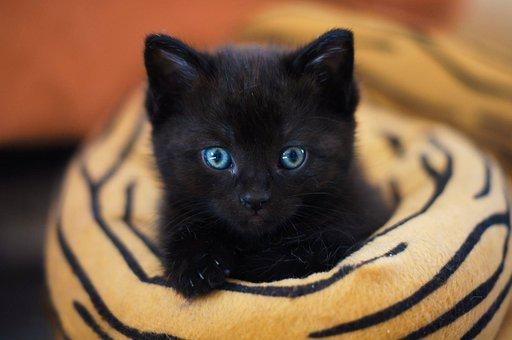
\includegraphics[width=0.3333\hsize]{./img/gatitoNegro}
    \caption{Un gato negro} %caption que se ve
    \label{fig:gatitoNegro} %nombre interno para referenciar luego
\end{figure}

Si ahora quieres referenciar una figura en un párrafo en \LaTeX puedes poner
\texttt{ \textbackslash ref\{nombre de la referencia\}}.
Por ejemplo: como podemos ver en la Figura \ref{fig:gatitoNegro}:
\nameref{fig:gatitoNegro}. A continuación, vamos a insertar una tabla.
% Esto no sirve para hacer la tabla en sí misma, sino para ponerle captions y
% esas cosas. Es equivalente a \begin{figure} que no inserta una imagen, pero
% nos prepara las cosas para que se comporte como una figura, así podemos
% ponerle título y referenciarla.
\begin{table}[H]
    % Aquí defines la tabla en sí misma, tienes que poner tantas letras como
    % columnas vaya a tener la tabla, y puedes poner líneas verticales entre
    % ellas escribiendo este símbolo entre las letras. Estas letras son los
    % especificadores de alineación. Si pones l, la columna se alinea a la
    % izquierda, si pones c, al centro, y si pones r, a la derecha.
    \begin{tabular}{|c|r|c|r|}
    % Esta orden genera una línea entre filas de la tabla.
    \hline
    % En las tablas las celdas se separan con & y las filas con \\
    % Puede haber celdas vacías, pero todas las filas deben tener las mismas
    % celdas.
    Concepto & Precio Unitario & Cantidad & Subtotal\\ \hline
    Placa base & \EUR{89.99} & 1 & \EUR{89.99}\\ \hline
    Memoria RAM 8GB DDR4 3200 MHz & \EUR{40.44} & 4 & \EUR{161.76} \\ \hline
    % Aquí podemos ver que hemos puedo celdas vacías. (dos & seguidos)
    \textbf{Total}&&&\textbf{\EUR{251.75}} \\ \hline
\end{tabular}
    % De nuevo, el título que se ve
    \caption{Gastos de la reparación}
    % La referencia interna. 
    \label{tab:gastos}
\end{table}

De nuevo, podemos referenciar el número de la tabla con \ref{tab:gastos} y su
títulos con \nameref{tab:gastos}. Nota del autor: a veces salen signos de
interrogación, no te preocupes, \LaTeX a veces necesita dos compilaciones para 
crear la base de datos de referencias.

Creo que ya estás listo para usar \LaTeX.
He incluido un fichero makefile en el directorio que debería compilar el 
archivo presente con la orden \texttt{pdflatex} dos veces.



\end{document}
